\subsection{A better distribution score need not locate the mean better}
The 300 s observation-interval procedure illustrates the distinction.
Relative to its named Full01 control, weighted ES changes by $-23.40$ m
but FDE by $+9.64$ m. Its mean-position error is also larger at each of the
four saved targets (Table~\ref{tab:point-errors}). ES accounts both for
distances to the target and for spread between particles; it cannot be
converted into mean-position error. The observation-interval comparison
changes training exposure and diffusion binding as well as cadence, so
this contrast does not isolate a numerical integration effect.

\begin{figure}[htbp]\centering
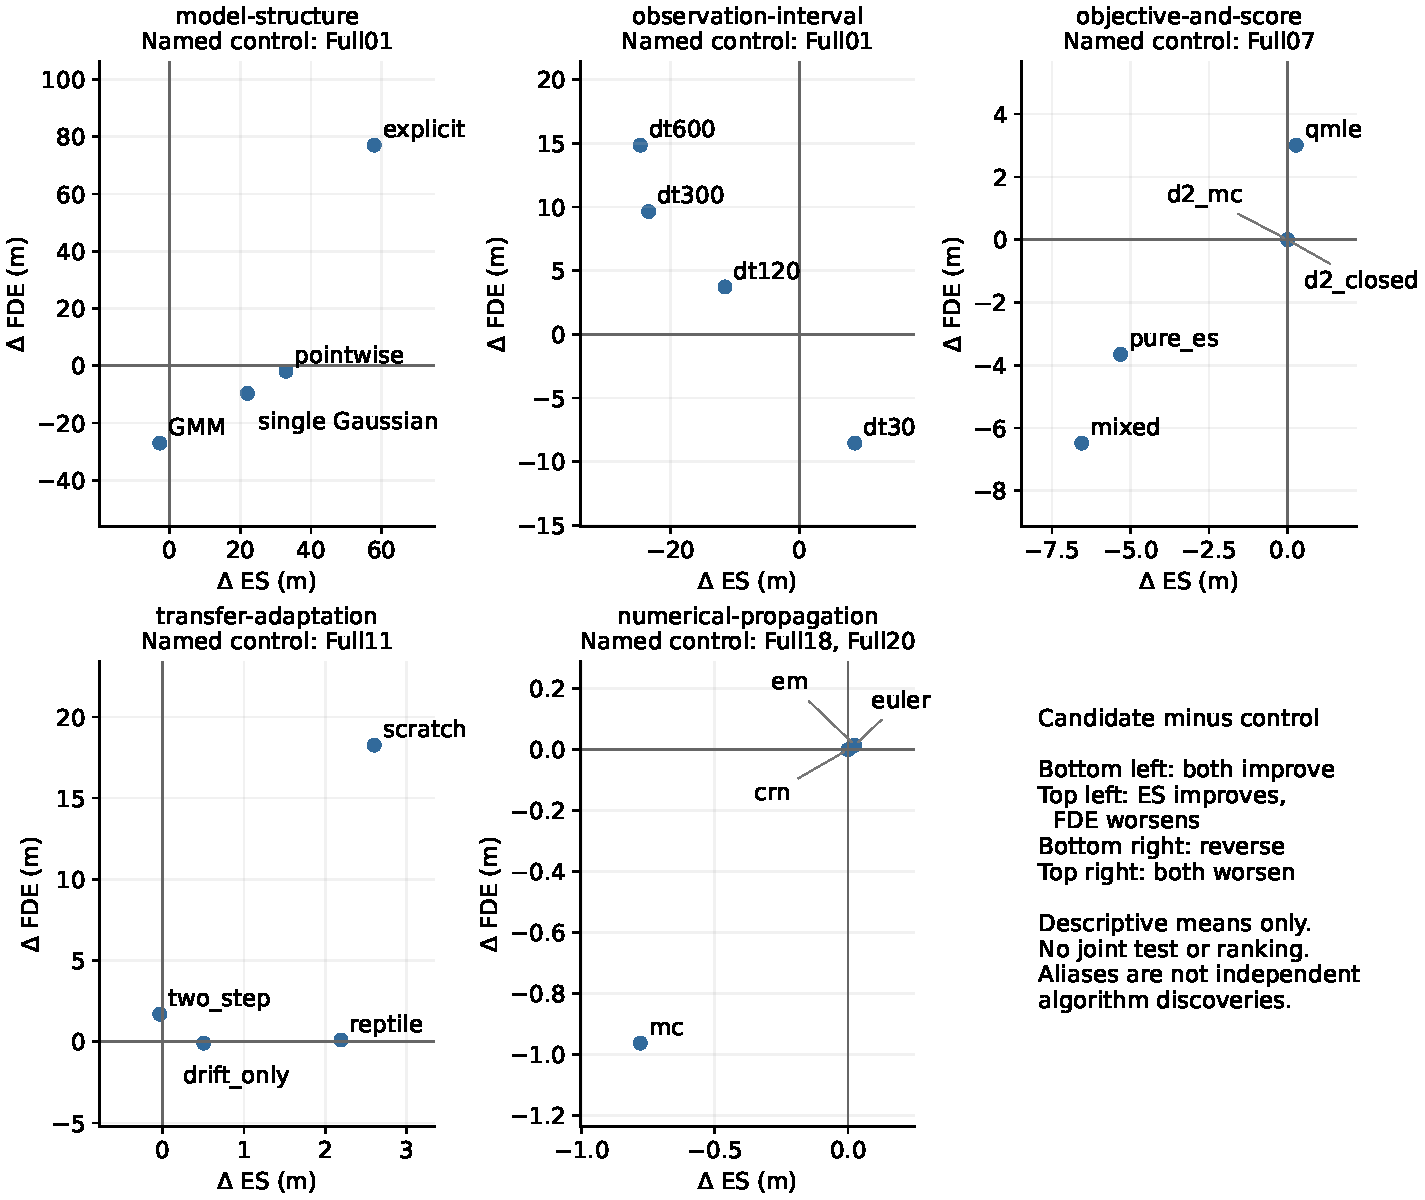
\includegraphics[width=\linewidth]{../figures/reader-v2/tradeoff.pdf}
\caption{Distribution-score versus endpoint-error trade-offs. All 21
comparisons (42 displayed scalar differences) retain five registered
families and named controls. Each point averages five simulation seeds
within each of 46 paired blocks, then weights blocks equally; ES first
averages four targets while FDE uses only the last. Negative is favourable
on both axes; the upper-left quadrant improves ES but worsens FDE. Facets
have different scales. These means have no joint confidence region and
do not establish a Pareto or global algorithm ranking.}
\label{fig:reader-tradeoff}\end{figure}
The dt300 ES simultaneous interval is $[-48.27,-2.47]$ m. Excluding zero
does not satisfy the registered practical-benefit criterion: the whole
interval would have to be below $-41.100259$ m, with the other gates met.
The point thus communicates a metric conflict, not a practically superior
method. All differences are calculated from unrounded source values.
\FloatBarrier
